

\chapter*{SVM-Simone Cogno}
Pour la reconnaissance du geste dans ce challenge, on pouvait choisir entre 3 différents algorithmes de machine learning. J'ai choisi SVM parce que c'était l'algorithme que j'avais compris le plus. j'avais le dut avec choisi ANN, mais a été choisi par mon collègue Marco. HMM il parait entre le plus adapté par la structure des données à traiter, mais ses détails d'implémentation n'est sont pas encore assai claire.

\section*{Prétraitement}
Dans la phase de prétraitement, il a été effectué une modification initiale de données brutes pour le mieux visualiser et pour le rendre plus lisible.
 Pour ce faire on a créé des Histogrammes pour chaque caractéristique.
Dans l'image \ref{fig:prehist} on peut voir, un histogramme fait en utilsiatn l'accélération de la main dans l'axe des X.

On peut voir que le range des valeurs va entre -1  jusqu'à 1 pour la majorité des points.
\begin{figure}[h]
  \centering
    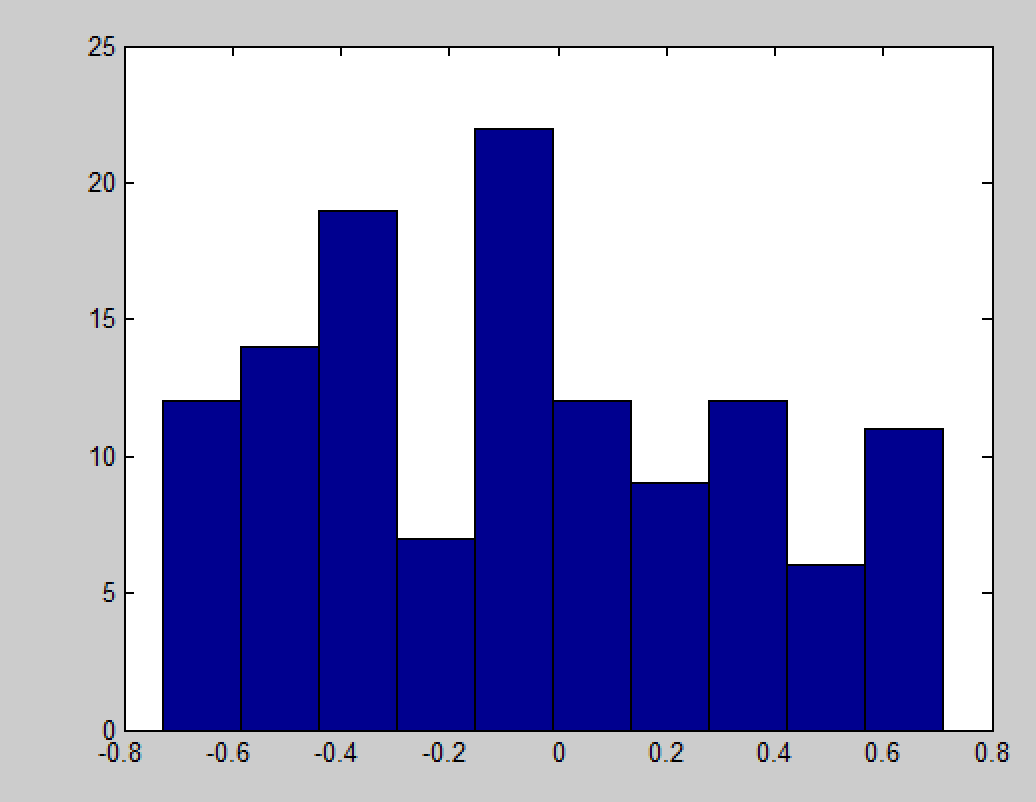
\includegraphics[width=0.5\linewidth]{img/pretraitement/hist10.png}
  \caption{histogramme du signal AccX de la class 1}
  \label{fig:prehist}
\end{figure}

En addition à la lisibilité du signal, un histogramme peut être très utile pour représenter un signal continu.

Sur les données des histogrammes une normalisation a été effectué pour éviter d'avoir de différence par rapport au nombre d'observations de chaque classe  et caractéristique.

Pour faire cela, on a divisé chaque valeur de l'histogramme par le nombre d'observations totales.

On peut voire dans la figure \ref{fig:normalization} que les deux histogrammes à gauche sont ont de valeur diffèrent, mais la forme est identique. Pour notre algorithme on ne s’intéresse pas aux valeurs elles-mêmes, mais plutôt à la forme de l'histogramme. Ces deux histogrammes douteraient être alors identique. La normalisation sur les valeurs fait exactement cela (histogrammes à gauche)

\begin{figure}[h]
  \centering
    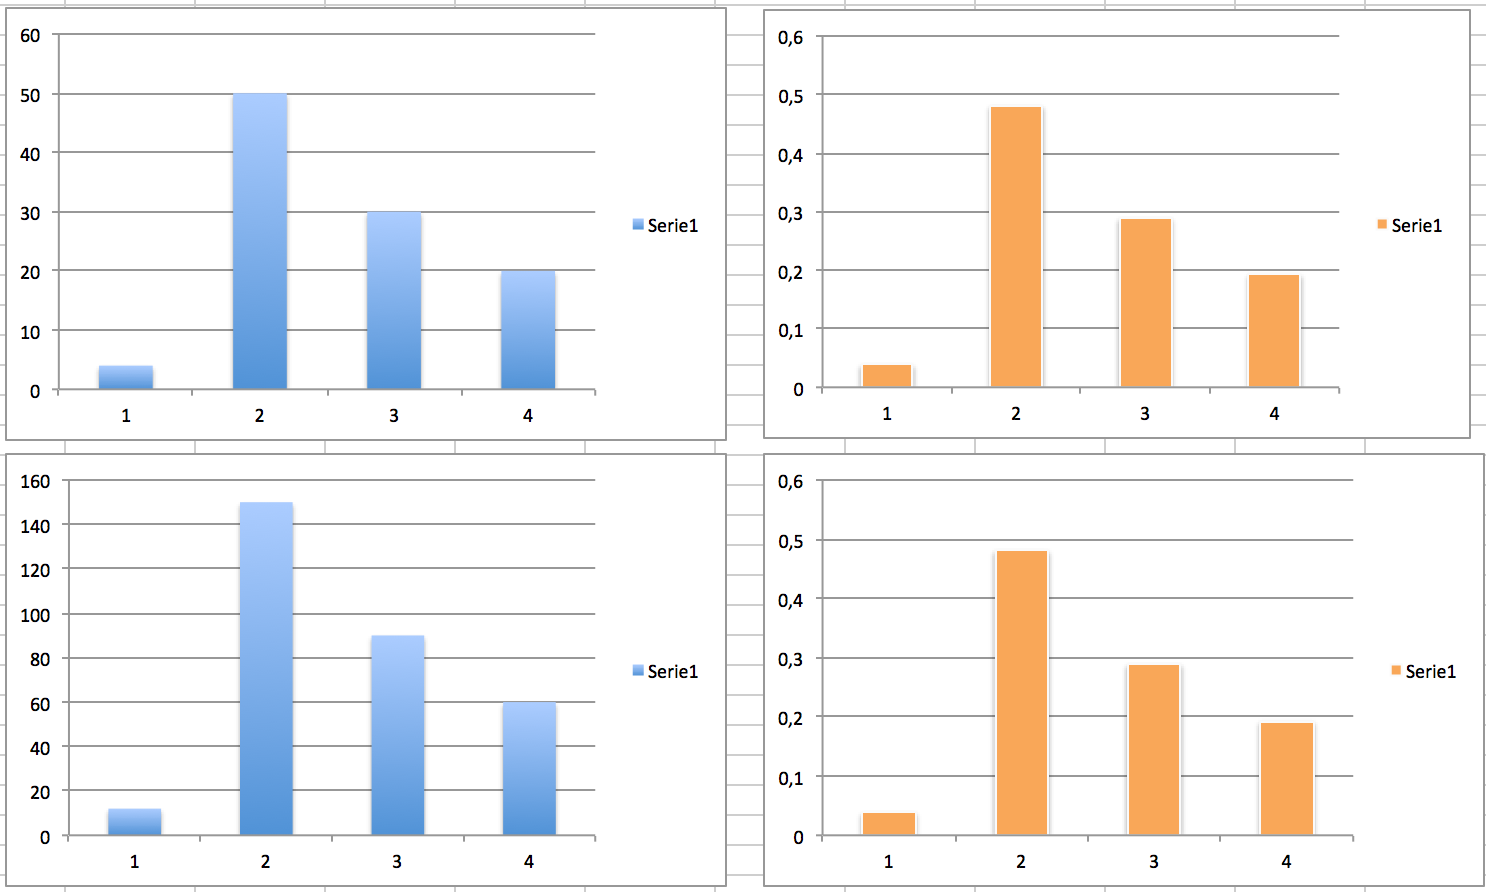
\includegraphics[width=0.8\linewidth]{img/pretraitement/normalization.png}
  \caption{Normalisation des valeurs des histogrammes}
  \label{fig:normalization}
\end{figure}


\section*{Extraction des caractéristiques}
Dans cette phase on a pu utiliser les histogrammes faits dans le prétraitement pour mieux comprendre les caractéristiques. Il a été effectué une comparaison entre plusieurs histogrammes faits sur le même signal, mais avec de classe différente. Dans l'image \ref{fig:histogram-pre} on peut voir que l'histogramme du signal AccX est assai différent pour les trois classes mises en évidence.

Ce signal puera donc entre un bon candidat pour différentier les différentes classes et pour entrainer notre modèle. 


\begin{figure}[h!]
    \centering
    \begin{tabular}{cccc}
      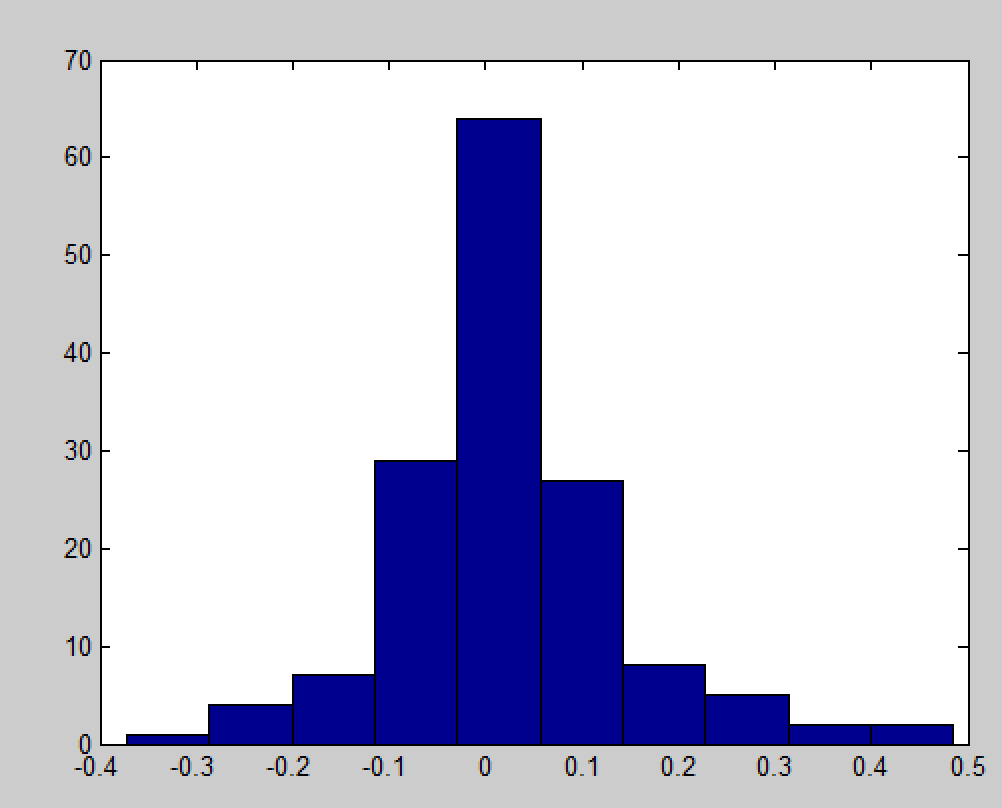
\includegraphics[width=.30\linewidth]{img/pretraitement/hist0.png} &
      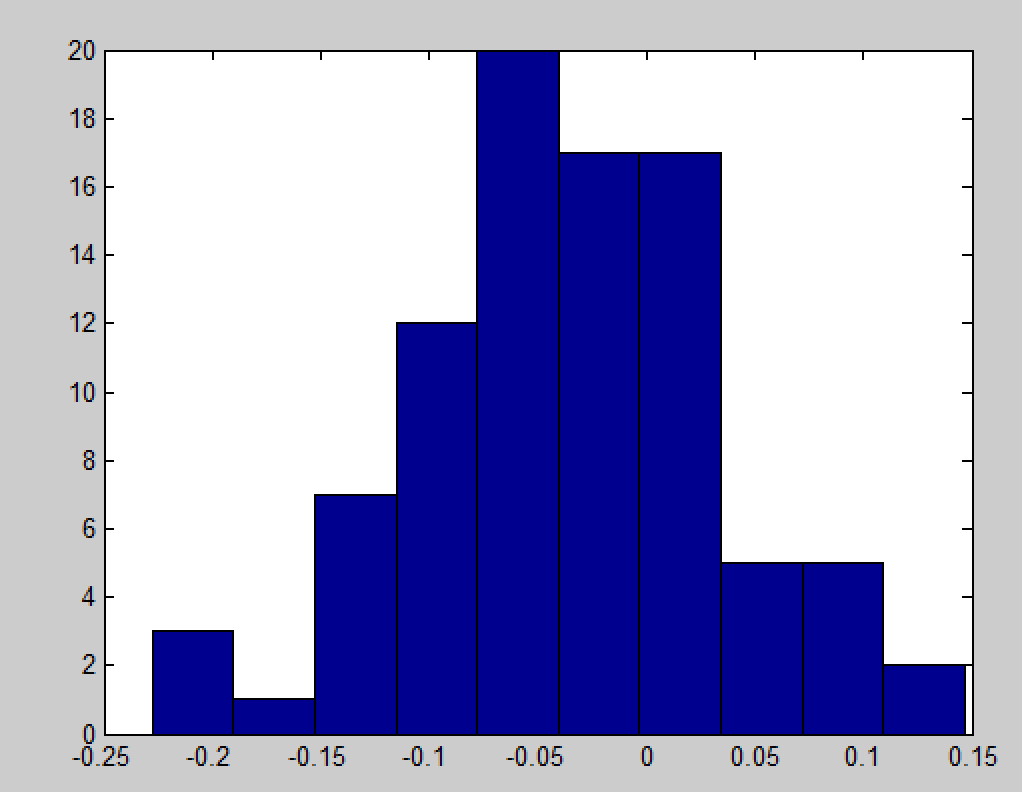
\includegraphics[width=.30\linewidth]{img/pretraitement/hist1.png} &
      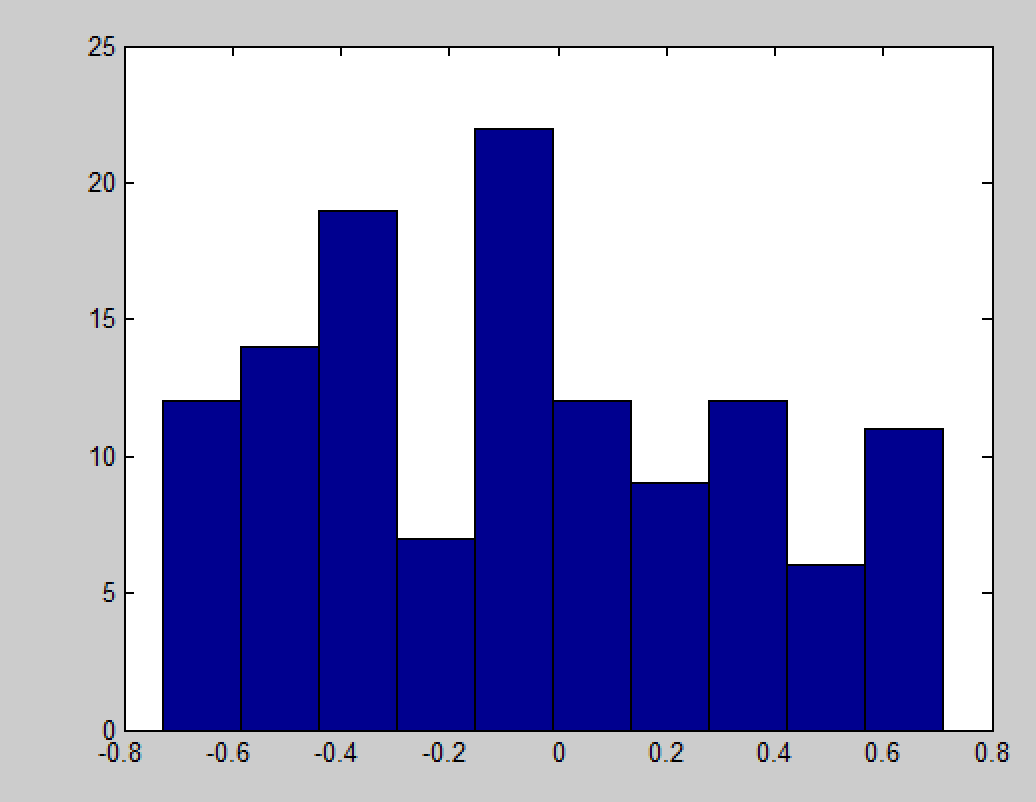
\includegraphics[width=.30\linewidth]{img/pretraitement/hist10.png} \\
      (a) & (b) & (c)\\
    \end{tabular}
    \caption{AccX pour les classes (a) 0 (b) 1 (c) 10
    \label{fig:histogram-pre}}
\end{figure}


En plus des l'"AccX" il a été utilise le "AccY", "AccZ" de la main et le "AccX","Z" du bracelet ainsi que le signal "Pinch" de la main.

Ces différents histogrammes  des caractéristiques ont été mis ensemble pour donner un unique vecteur des caractéristiques. 

Une visualisation des histogrammes mis ensemble pour quatre différentes classes est montrée dans l'image \ref{fig:histvector}. Dans cette figure sont montrées toutes les occurrences de chaque classe.

\begin{figure}[h]
  \centering
    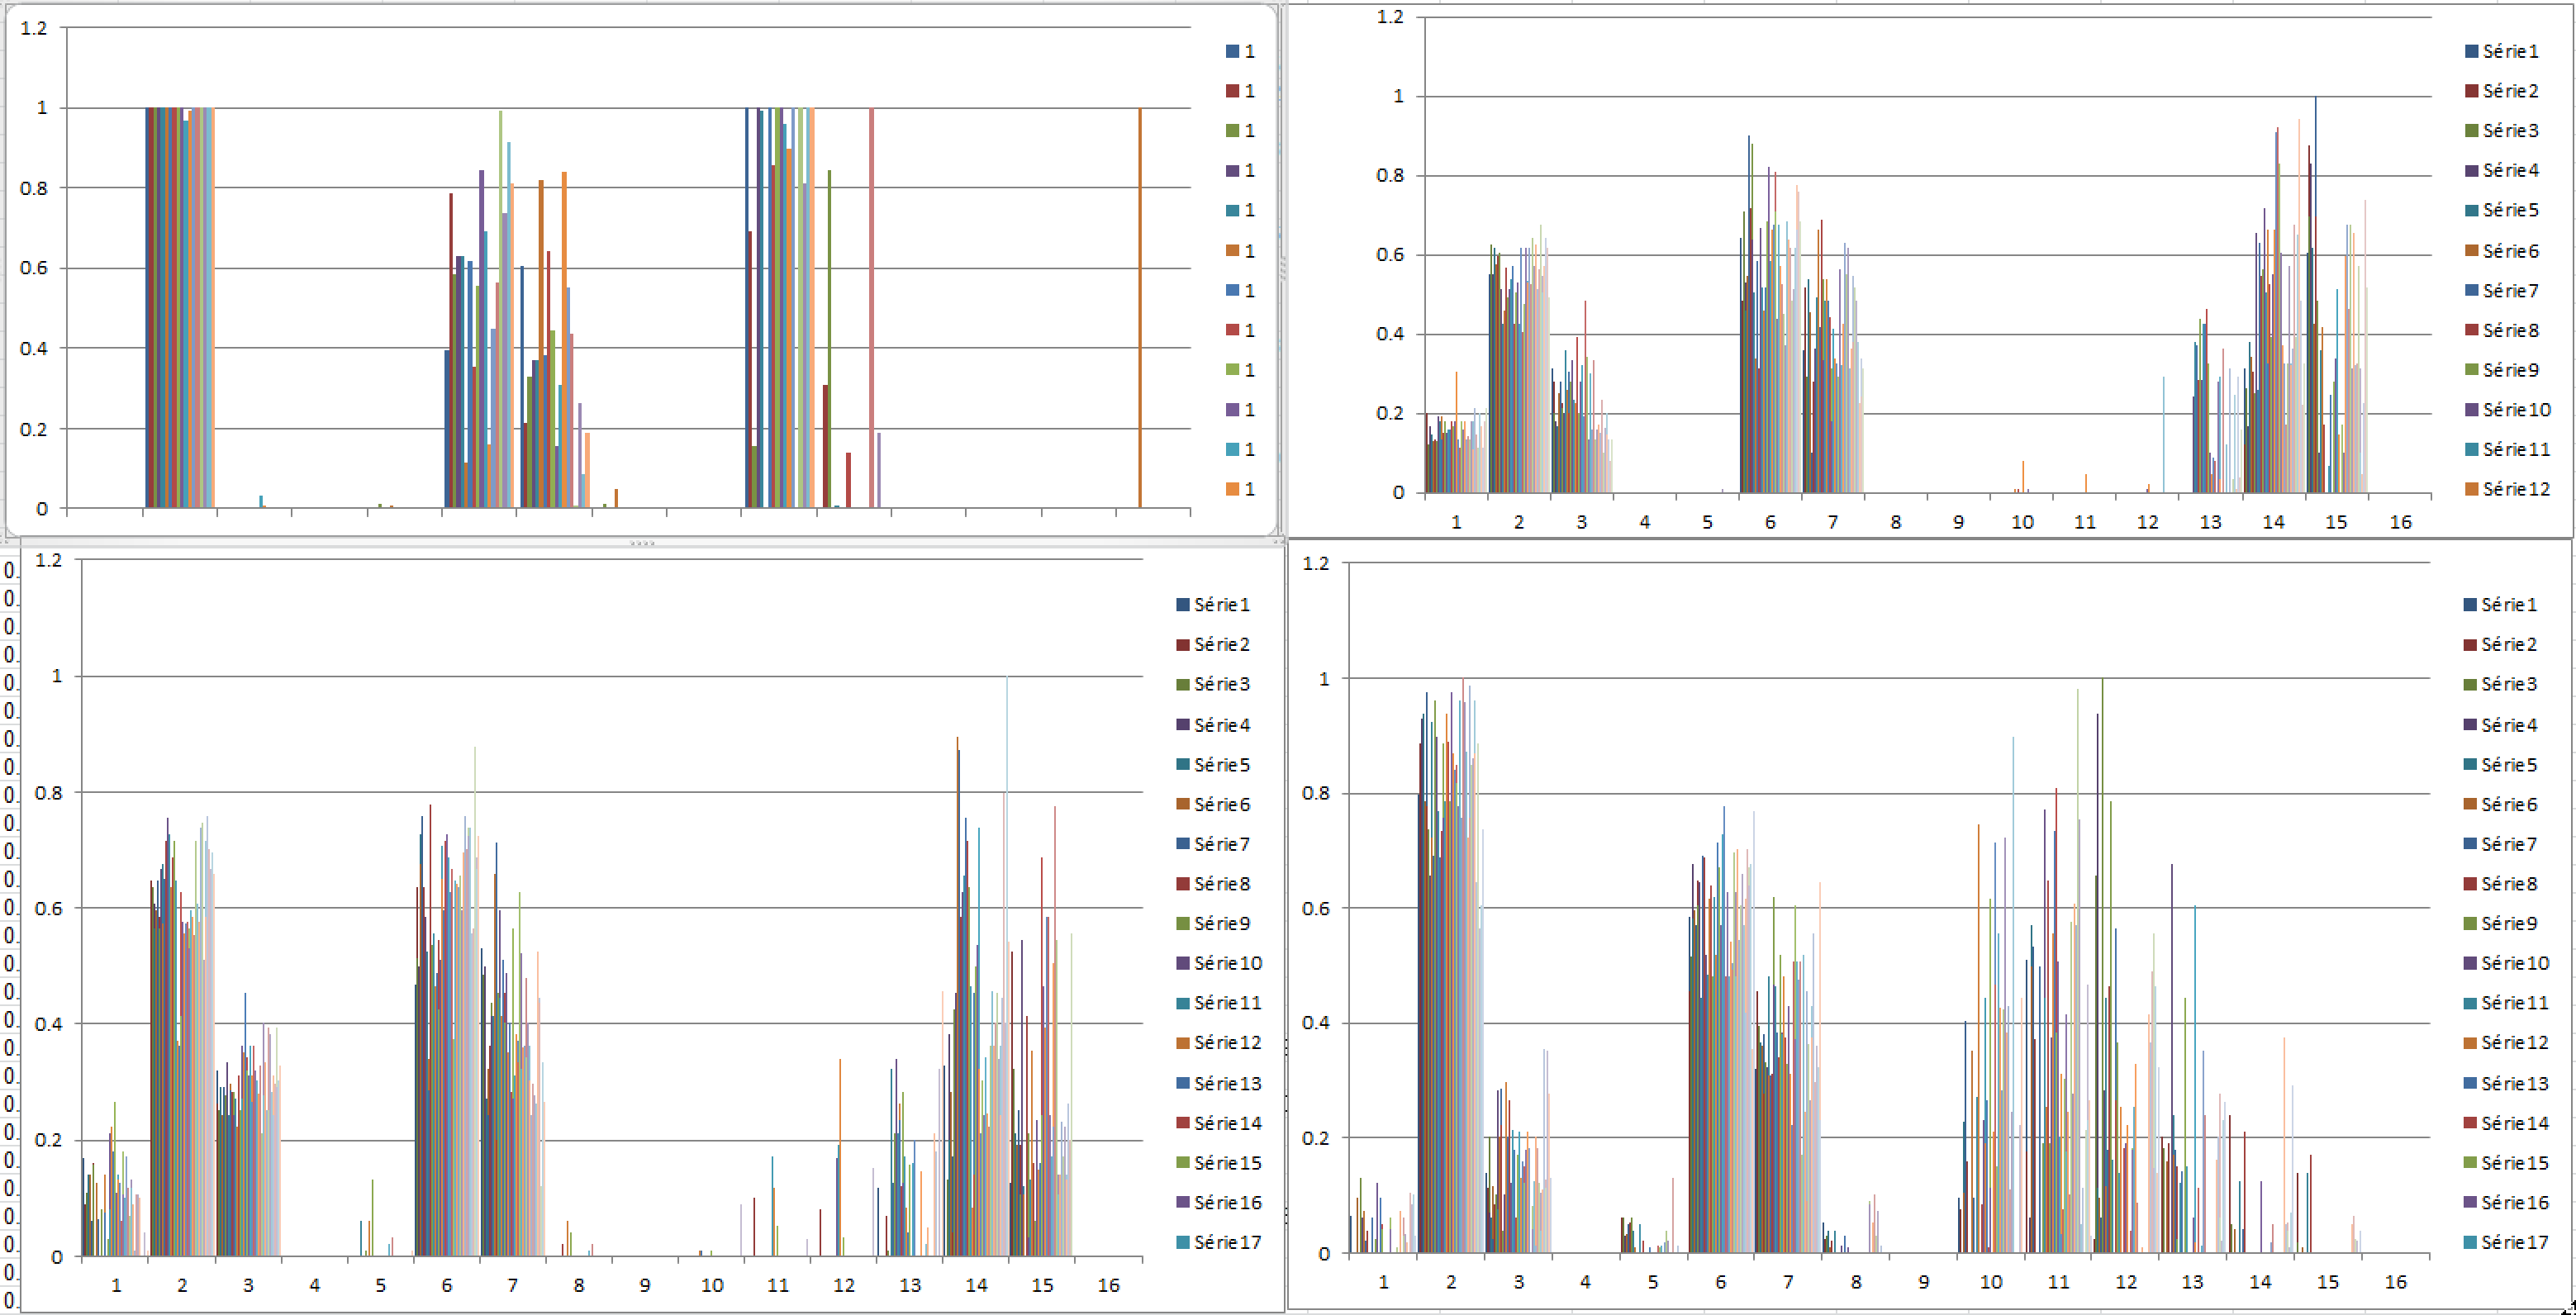
\includegraphics[width=1\linewidth]{img/extraction/vector-hist.png}
  \caption{Group of histogrammes représentant quatre different classes}
  \label{fig:histvector}
\end{figure}

O peut voir depuis cette figure que la forme des histogrammes est presque identique pour le même geste. Par contre il est assis diffèrent par rapport les outres geste.

\section*{Entrainement}

Pour entrainer le SVM on a besoin d'une matrice où chaque ligne représente un geste et chaque colonne une caractéristique. Dans notre cas pour chaque histogramme, on a plus ou moins 10 caractéristiques qui sont représentées par un nombre de 0 à 1.  Ces caractéristiques sont en effet les bins des histogrammes.

Pour entrainer notre modèle avec un SVM binaire il a été cecessaire d’ entrainer et créer plusieurs modèles: un modèle par classe. En faisons cela chaque modèle est capable de reconnaitre une seule classe.

La démarche d'entrainement sera donc la suivante:
\begin{lstlisting}[language=python]
    for i=1:NUM_CLASSES %Train model for all classes
        label=(Y==i); %Convert multi class to double class 1 or 0
        svmStructs(i) = svmtrain(X,label,'kernel_function','polynomial');
    end  %code insipred to multiclass svm
\end{lstlisting}


Pour entrainer et tester en locale l'algorithme, le set d'entrainement a été divisé en deux parties. Le premier a été utilisé pour entrainer le modèle et le deuxième pour tester en locale(figure \ref{fig:trainset}). Le test final e été fait directement sur la plateforme Opegra.

\begin{figure}[h]
  \centering
    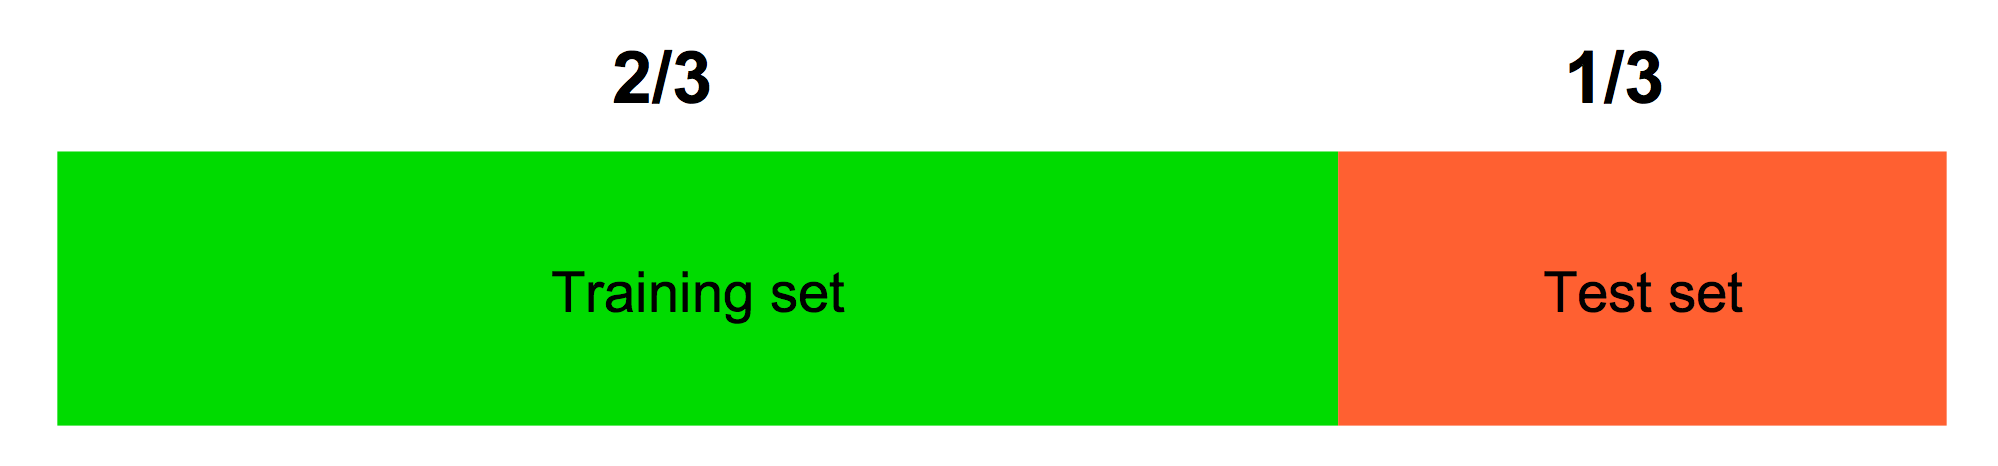
\includegraphics[width=1\linewidth]{img/evaluation/trainset.png}
  \caption{Découpage du set d'entrainement et de test}
  \label{fig:trainset}
\end{figure}



\section*{Évaluation}
L'évaluation des données de tests a été effectuée en utilisant les modèles créés durant l'entrainement. Pour utiliser un SVM binaire pour reconnaitre plusieurs classes on fait une évaluation de chaque modelé avec le geste du test. La classe de test sera identifiée quand un de ces modèles répond positivement.

Le diagramme \ref{fig:models-svm} montre en manière schématique comment cet algorithme fonctionne, on peut, voir que chaque entrée sera évaluée par chaque modèle SVM jusqu'à un modèle le reconnait.

Le problème de cette méthode est que si aucun des modelés ne reconnait la classe d'une instance de tests, une valeur par défaut lui sera attribuée, dans notre case la classe 10.

Cela, ça peut devenir un problème quand les gestes seront nombreux et similaires entre eux. Une manière pour améliorer cela puera être d'attribuer un score à chaque évaluation de classe et finalement choisir celle avec le plus grand score.


\begin{figure}[h]
  \centering
    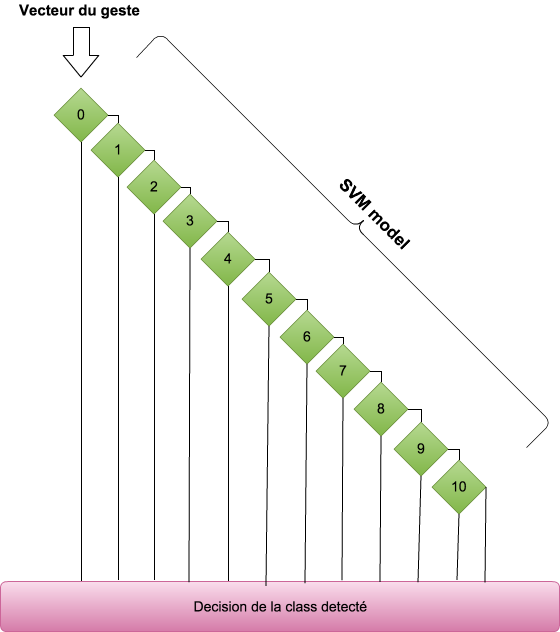
\includegraphics[width=0.7\linewidth]{img/evaluation/svm-class.png}
  \caption{Matrice de confusion de l'évaluation des gestes de test}
  \label{fig:models-svm}
\end{figure}


\section*{Résultats obtenus}
Dans la matrice de confusion obtenue depuis l'évaluation du set de test  (figure \ref{fig:conferror})  on peut voire que les classes sont assai bien classifier parce que sont distribué pour la plupart sur la diagonale. Le F1-Score de ce algorithme ainsi que ce score total dans Opegra est de \textbf{0.86}.

Par contre il a encore quelque geste que l'algorithme est indécis entre deux gestes similaires et il a encore beaucoup d'erreurs de reconnaissance. On voit par exemple que l'algorithme a une certaine difficulté a différencier le geste right/left et push/pull.

On voit aussi que beaucoup d'erreurs sont dans la class 11. Comme explique dans la section précédente c'est en effet les  lasse que ne son pas reconnu par les modelés entrainés.



\begin{figure}[h]
  \centering
    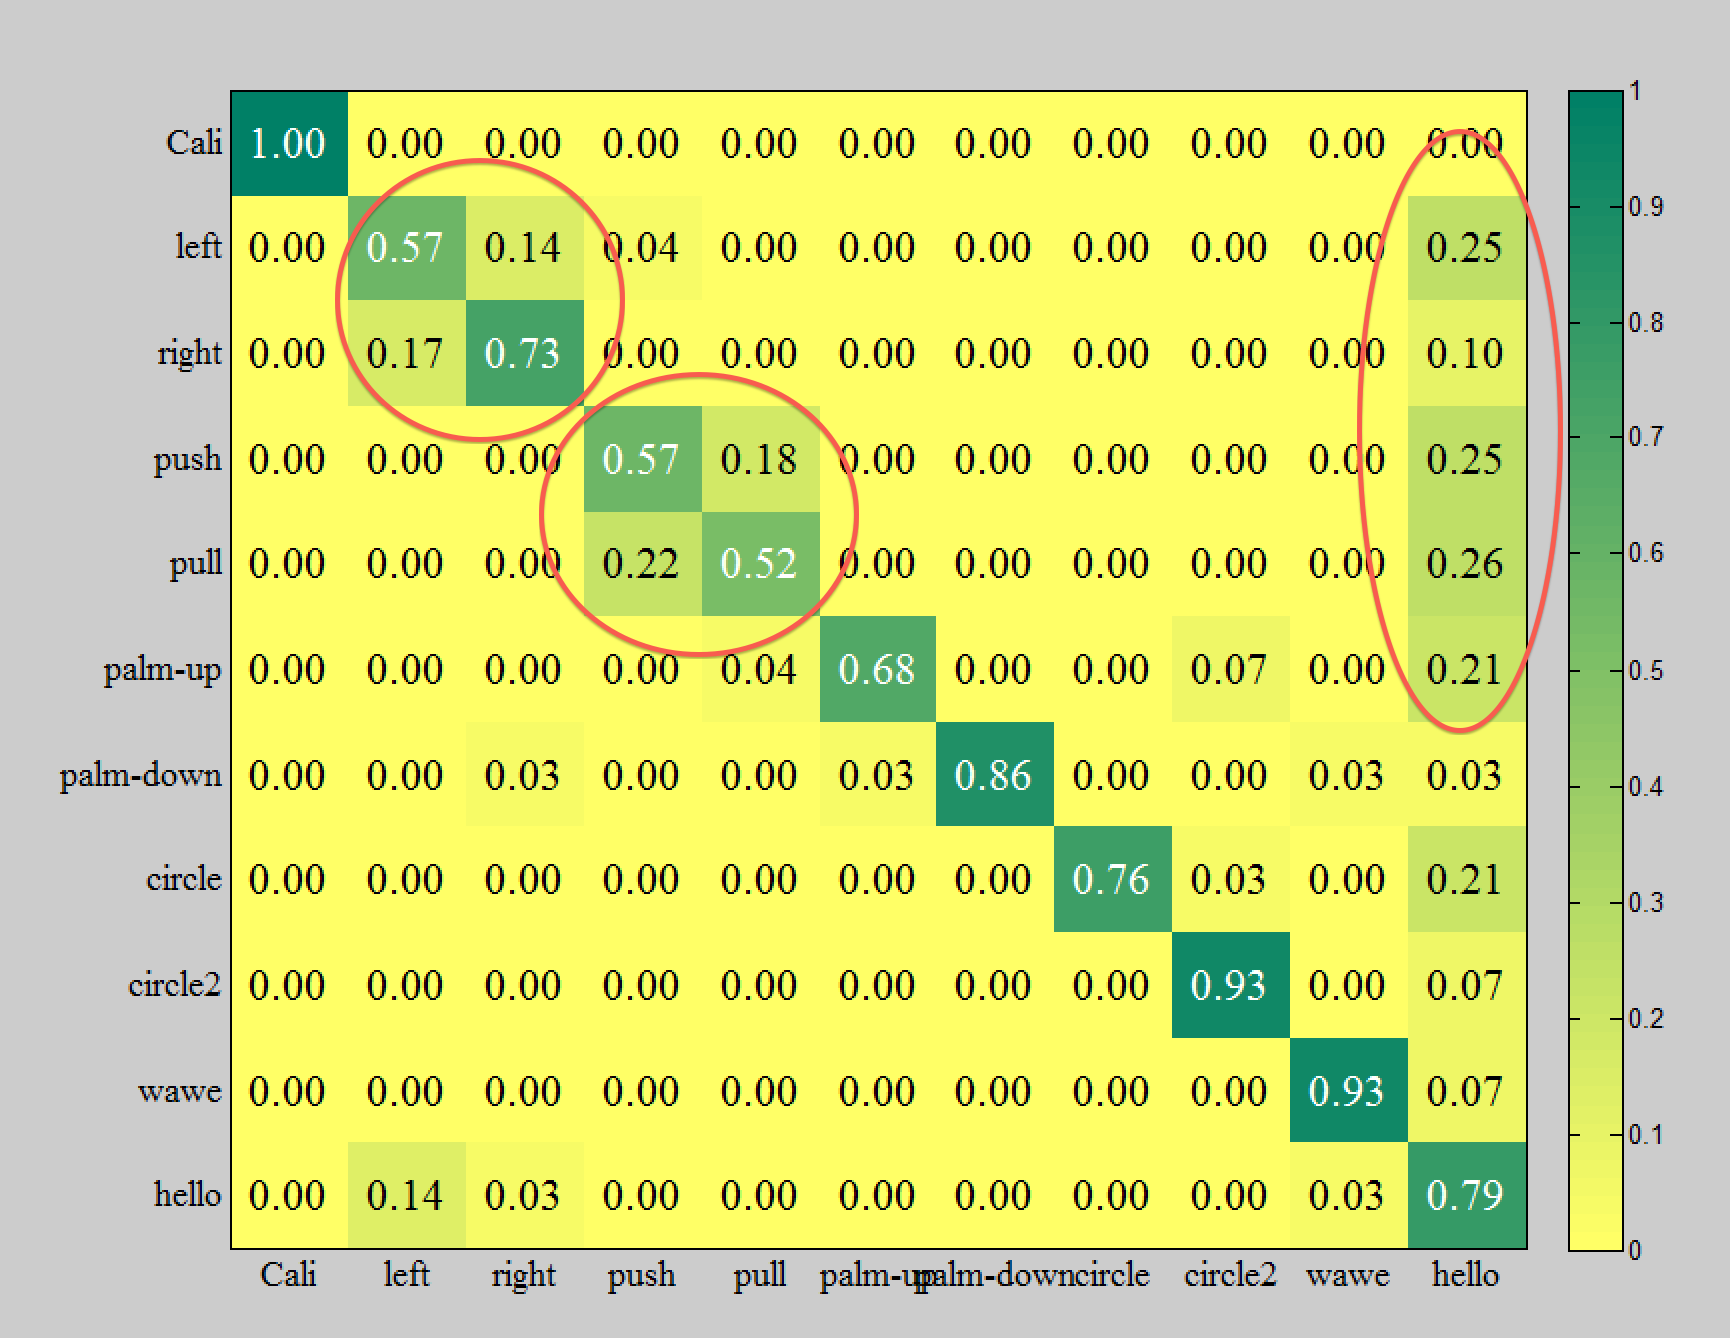
\includegraphics[width=0.7\linewidth]{img/evaluation/evalerror.png}
  \caption{Matrice de confusion de l'évaluation des gestes de test}
  \label{fig:conferror}
\end{figure}

\section*{Problèmes rencontrés}
Dans la première version de l'algorithme a été utilisé Fitcecoc comme fonction d'entrainement pour l'algorithme SVM. Après avoir appris que cette fonction n'étés pas supportée par la plateforme Opegra \footnote{Opegra,\url{https://project.eia-fr.ch/chairgest/Pages/Opegra/Download.aspx}}. J’ai recherché sur internet une fonction similaire qui était compatible avec Matlab 2014. J'ai donc trouvé la fonction DSVM   \footnote{DVSM,\url{http://www.mathworks.com/matlabcentral/fileexchange/downloads/68289/akamai/DSVM.zip}} Mais ce script il faisait une erreur quand on faisait un entrainement avec plus que 6 classes comme montré dans l'image \ref{fig:dsvm}. 

Ensuite a version similaire a le multiclass SVM \footnote{Multiclass SVM,\url{http://www.mathworks.com/matlabcentral/fileexchange/33170-multi-class-support-vector-machine}} a été implémenté même si n'est pas une solution définitive.


J'ai aussi rencontré quelque problème a intégrer les données de la kinect, mais,  vu le nombre d'observations différentes par rapport au dataset su xsens je n'ai pas réussi a l’ implémenter.


 

\section*{Perspectives et améliorations}
Certaines améliorations pouvant être effectuées sur la partie d'entrainement de l'algorithme SVM. Par exemple, il sera envisageable d’ implémenter un k-fold cross validation pour l'entrainement des nos modèles. 
Une extraction des caractéristiques plus avancée pourra aussi être effectuée sur les données par exemple avec une analyse FFT.
Ensuite une amélioration de l’ algorithme multiclass SVM pourra être effectuée en définissant un score à chaque évaluation pour évier d'avoine des classes pas détectées.

Bien sûr un meilleur choix des caractéristiques utilisé dans l'algorithme sera aussi très important pour améliorer le score de reconnaissance de l'algorithme.

\section*{Conclusion}
En conclusion l'algorithme SVM utilisé pour cette expérience fonctionne bien avec les caractéristiques et le prétraitement effectué sur le données. Il a été  atteint un F1-Score de 0.86 qui est suffisant pour un algorithme de ce type. C'est évidant que sera encore améliorable avec un entrainement plus précis, une extraction des caractéristiques plus avancées et un choix et une analyse plus détaillée sur les caractéristiques à utiliser pour différencier les différents gestes.








% Code integration example
%\begin{lstlisting}[language=bash]
%  sudo apt-get update
%  sudo apt-get install drupal7
%\end{lstlisting}

% Image integration example
%\begin{figure}[h]
%  \centering
%    \includegraphics[width=1\linewidth]{img/drupalFirstPage.png}
%  \caption{Page d'accueil du site créé avec Drupal sur une instance EC2}
%  \label{drupalfirstpage}
%\end{figure}

% Image side-by-side
%\begin{figure}[h!]
%    \centering
%    \begin{tabular}{cccc}
%      \includegraphics[width=.14\linewidth]{randomTree_n5.png} &
%      \includegraphics[width=.22\linewidth]{randomTree_n10.png} &
%      \includegraphics[width=.22\linewidth]{randomTree_n15.png} \\
%      (a) & (b) & (c)\\
%    \end{tabular}
%    \caption{Arbres aléatoires où (a) n=5 (b) n=10 (c) n=15
%    \label{randomTrees}}
%\end{figure}
